\documentclass[9pt]{beamer}
\usetheme{Madrid}
\usepackage{hyperref}
\usepackage{tikz}
\usetikzlibrary{arrows.meta,positioning}

% 设置全局字号
\setbeamerfont{normal text}{size=\scriptsize}
\setbeamerfont{title}{size=\Large}
\setbeamerfont{frame title}{size=\normalsize}
\setbeamerfont{block title}{size=\small}
\setbeamerfont{itemize/enumerate body}{size=\footnotesize}

% 减少列表间距
\setlength{\itemsep}{2pt}
\setlength{\parsep}{1pt}

% 为所有frame设置更紧凑的布局
\setbeamersize{text margin left=0.5cm,text margin right=0.5cm}

% 设置块内容字号
\setbeamerfont{block body}{size=\footnotesize}

\title{Progress Report\\\vspace{0.3em}Interface Fuzzing for Isabelle/Sledgehammer}
\subtitle{Knowledge Exchange Projects - Amazon — Variant 3}
\author{Qilan Lin (K21204786)}
\institute{King's College London}
\date{21\textsuperscript{st} November 2025}

\begin{document}

%------------------------------------------------
% Slide 1: Title
%------------------------------------------------
\begin{frame}
  \titlepage
  \vspace{-0.5cm}
  \begin{center}
  \textbf{Project Description:} Fuzzing the interface between Isabelle/HOL's Sledgehammer and external ATP/SMT provers to improve reliability and discover integration bugs.
  \end{center}
\end{frame}

%------------------------------------------------
% Slide 2: Current State (What you have achieved)
%------------------------------------------------
\begin{frame}{Current State of Project}
\begin{block}{Overall Progress: 25\% Complete — \textcolor{green}{On Track}}
\begin{center}
\scalebox{0.7}{
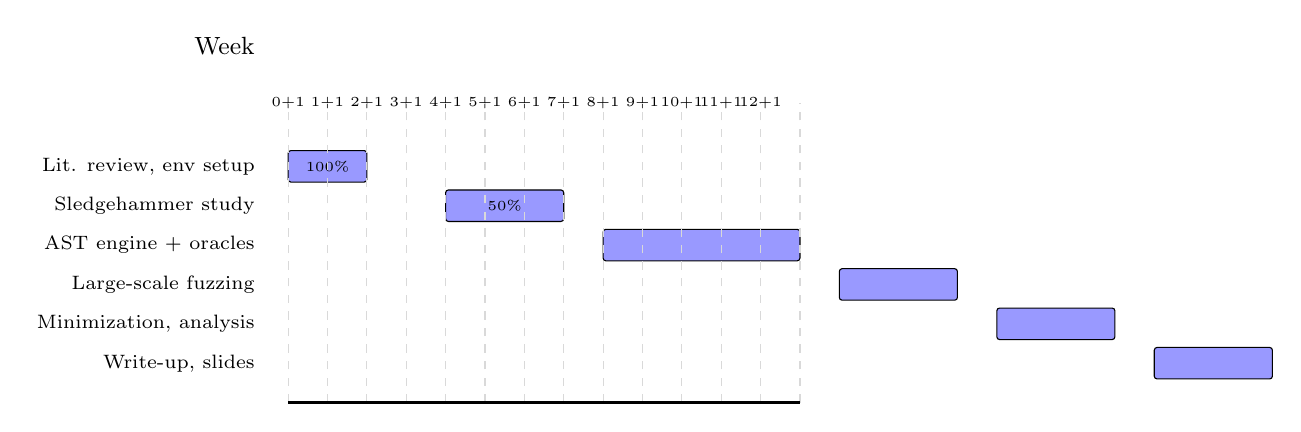
\begin{tikzpicture}[
    ganttbar/.style={draw, fill=blue!40, minimum height=0.5cm, rounded corners=1pt},
    ganttlabel/.style={anchor=east, font=\scriptsize},
    weeklabel/.style={font=\tiny, anchor=north}
]
    % Week labels (x-axis)
    \foreach \x in {0,...,12} {
        \node[weeklabel] at (\x*0.5, 5.5) {\x+1};
    }
    \node[anchor=south east, font=\small] at (-0.3, 5.8) {Week};
    
    % Task 1: Literature review, environment setup (Week 1-2)
    \node[ganttlabel] at (-0.3, 4.5) {\scriptsize Lit. review, env setup};
    \draw[ganttbar] (0, 4.3) rectangle (1, 4.7);
    \node[font=\tiny] at (0.5, 4.5) {100\%};
    
    % Task 2: Sledgehammer study (Week 3-4)
    \node[ganttlabel] at (-0.3, 4.0) {\scriptsize Sledgehammer study};
    \draw[ganttbar] (2, 3.8) rectangle (3.5, 4.2);
    \node[font=\tiny] at (2.75, 4.0) {50\%};
    
    % Task 3: AST engine + oracles (Week 5-7)
    \node[ganttlabel] at (-0.3, 3.5) {\scriptsize AST engine + oracles};
    \draw[ganttbar] (4, 3.3) rectangle (6.5, 3.7);
    
    % Task 4: Large-scale fuzzing (Week 8-9)
    \node[ganttlabel] at (-0.3, 3.0) {\scriptsize Large-scale fuzzing};
    \draw[ganttbar] (7, 2.8) rectangle (8.5, 3.2);
    
    % Task 5: Minimization, analysis (Week 10-11)
    \node[ganttlabel] at (-0.3, 2.5) {\scriptsize Minimization, analysis};
    \draw[ganttbar] (9, 2.3) rectangle (10.5, 2.7);
    
    % Task 6: Write-up, slides (Week 12-13)
    \node[ganttlabel] at (-0.3, 2.0) {\scriptsize Write-up, slides};
    \draw[ganttbar] (11, 1.8) rectangle (12.5, 2.2);
    
    % Grid lines
    \foreach \x in {0,...,13} {
        \draw[gray!30, dashed] (\x*0.5, 1.5) -- (\x*0.5, 5.3);
    }
    \draw[thick] (0, 1.5) -- (6.5, 1.5);
\end{tikzpicture}
}
\end{center}
\end{block}

\begin{block}{Achievements Since Last Meeting}
\begin{itemize}\footnotesize
  \item ✓ \textbf{Week 1-2 Complete (100\%)}: Environment setup, tool installation, 480 TPTP seed files extracted
  \item ✓ \textbf{Week 3-4 Progress (50\%)}: MVP framework implemented (7 modules, $\sim$1100 LOC)
    \begin{itemize}\tiny
      \item TPTP parser, token mutator (8 operations), crash/hang oracle, differential oracle
      \item Statistics and logging utilities, main fuzzer program
    \end{itemize}
  \item ✓ \textbf{Testing \& Enhancement}: 644 test cases run successfully (100\% success rate)
    \begin{itemize}\tiny
      \item Mutator enhanced from 5 to 8 operations (+60\%)
      \item Generation rate improved by 41\%, performance by 39\%
    \end{itemize}
\end{itemize}
\end{block}
\end{frame}

%------------------------------------------------
% Slide 3: Current Barriers
%------------------------------------------------
\begin{frame}{Current Barriers \& Challenges}
\begin{block}{Technical Barriers}
\begin{itemize}\footnotesize
  \item \textbf{Remaining Week 3-4 tasks (50\%)}:
    \begin{itemize}\tiny
      \item Code optimization and parallel processing not yet implemented
      \item Additional mutation strategies needed for better bug discovery
    \end{itemize}
  \item \textbf{Week 5-7 not started}: AST-level mutator and reconstruction oracle pending
    \begin{itemize}\tiny
      \item Requires deeper understanding of pySMT AST structure
      \item Need to integrate Isabelle/Sledgehammer output parsing
    \end{itemize}
\end{itemize}
\end{block}

\begin{block}{No Bugs Found Yet}
\begin{itemize}\footnotesize
  \item ✓ Framework is stable (644 tests, 0 crashes/timeouts)
  \item ⚠️ Current token-level mutations may not be aggressive enough
  \item \textit{Next step}: Implement AST-level mutations for deeper interface testing
\end{itemize}
\end{block}

\begin{block}{Progress Assessment}
\begin{itemize}\footnotesize
  \item \textcolor{green}{✓ On schedule}: Week 1-2 (100\%), Week 3-4 core (50\%) completed
  \item \textcolor{orange}{⚠️ Need acceleration}: Should start Week 5-7 preparation now
\end{itemize}
\end{block}
\end{frame}

%------------------------------------------------
% Slide 4: Planned Next Steps
%------------------------------------------------
\begin{frame}{Planned Next Steps}
\begin{block}{Immediate (Next 2 Weeks)}
\begin{itemize}\footnotesize
  \item \textbf{Complete Week 3-4 remaining tasks}:
    \begin{itemize}\tiny
      \item Code optimization and parallel processing
      \item Performance tuning and visualization tools
    \end{itemize}
  \item \textbf{Start Week 5-7 preparation}:
    \begin{itemize}\tiny
      \item Research pySMT AST structure and API
      \item Design AST mutator architecture
    \end{itemize}
\end{itemize}
\end{block}

\begin{block}{Short-term (Weeks 5-7)}
\begin{itemize}\footnotesize
  \item Implement AST-level mutator (structure-aware mutations)
  \item Implement reconstruction oracle (detect proof reconstruction failures)
  \item Create end-to-end prototype with all three oracles
\end{itemize}
\end{block}

\begin{block}{Long-term (Weeks 8-13)}
\begin{itemize}\footnotesize
  \item Large-scale fuzzing campaigns (all 480 seeds)
  \item Bug minimization, triage, and analysis
  \item Final report and presentation preparation
\end{itemize}
\end{block}

\begin{center}
\textbf{Target: Complete Week 3-4 by end of month, start Week 5-7 in December}
\end{center}
\end{frame}

\end{document}

